\documentclass[12pt, french]{article}

\usepackage{fancyhdr, fancybox, lastpage}
\usepackage[most]{tcolorbox}
\usepackage[a4paper, margin={0.3in, .75in}]{geometry}
\usepackage{wrapfig}
\pagestyle{fancy}
\renewcommand\headrulewidth{1pt}
\renewcommand\footrulewidth{1pt}
\fancyhf{}
\rhead{ \em{Zakaria Haouzan}}
\lhead[C]{\em{2ére année baccalauréat Sciences Mathématiques}}
\chead[C]{}
\rfoot[C]{}
\lfoot[R]{}
\cfoot[]{\em{Page \thepage / \pageref{LastPage}}}


\newtcolorbox{Box2}[2][]{
                lower separated=false,
                colback=white,
colframe=white!20!black,fonttitle=\bfseries,
colbacktitle=white!30!gray,
coltitle=black,
enhanced,
attach boxed title to top left={yshift=-0.1in,xshift=0.15in},
title=#2,#1}


\begin{document}
\begin{center}
   \shadowbox {\bf{ Soutien en physique et chimie}}
\end{center}


%%_________________________Exercice 5 : _________________________Exercice
\begin{Box2}{Exercice 1 : Mécanique }
Un skieur de masse m = 100 kg (équipement compris) est tiré par un bateau à l'aide d'une corde parallèle à la surface de l'eau. 
\begin{center}
    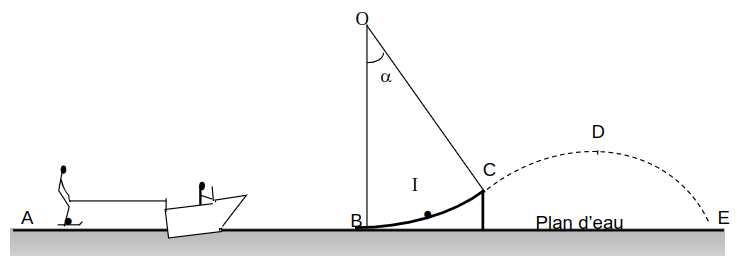
\includegraphics[width=1\textwidth, height =0.2\textwidth ]{./img/img01.png}
  \end{center}
Dans tout le problème, par souci de simplification on représentera les forces appliquéesau système \{skieur + skis\}  au niveau des skis

Données :$g = 10 N.kg^{-1}$ , $L = AB = 200 m$ ,  $\alpha=$30° ,  $OB = OC = 15 m$

   \underline{ \textbf{ $1^{\grave{e}re}$ étape (trajet AB): } } Le skieur démarre sans vitesse initiale du point A. Il est tracté par la force $\vec{F}$ constante et l’ensemble des forces de frottement est représenté par la force $\vec{f}$ d’intensité 100 N.Après un parcours de 200 m, le skieur atteint une vitesse $v_B= 20 m.s^{-1}$. 
\vspace{0.3cm}
\\1. Faire le bilan des forces s’exerçant sur le système \{skieur+skis\} sur la partie $A_B$.

2. Enoncé le théorème de l’énergie cinétique.

3. Exprimer les travaux des forces s’exerçant sur le système sur le trajet AB.

4. En déduire l’expressionla force de traction $\vec{F}$ en fonction de m, L, f, $v_B$.

5. Faire l’application numérique

\vspace{0.2cm}

   \underline{  \textbf{ $2^{\grave{e}me}$ étape (trajet BC):}} Le skieur lâche la corde en B et parcourt le tremplin BC qui est circulairede centre O de rayon OB = 15 m. OC fait un angle de 30° avec la verticale.Le tremplin est considéré comme parfaitement glissant.

\vspace{0.2cm}
6. Représenter sur le schéma au point I, les forces s’exerçant sur le système entre les points B et C (leurs caractéristiques ne sont pas demandées).

7. Exprimer la hauteur h acquise en haut du tremplin enfonction de OB et $\alpha$.

8. En appliquant le théorème de l’énergie cinétique, exprimer la vitesse $v_C$du skieur au point C en fonction de $v_B$, $\alpha$, g et OB.

9.Faire l’application numérique.

\vspace{0.2cm}
   \underline{  \textbf{ $3^{\grave{e}me}$ étape (trajet CE):}}Le skieur effectue un saut et retombe sur ses skis au point Ei Sur ce trajet, on supposera comme négligeable les frottements de l’air . La vitesse du skieur au point C est:  $v_C= 19 m.s^{-1}$ On prendra l’origine des altitudes en A.

10. Calculer l’énergie potentielle de pesanteur et l’énergie cinétique au point C.

11. La somme $E_c$ + $E_p$ est-elle constante entre C et E ? Justifier.

12. Représenter sur un graphique les variations des énergies cinétique et potentielle de pesanteur du skieur en fonction du temps sur le trajet CE. Justifier soigneusement l’allure des deux courbes.

13. La valeur de la vitesse au point D n’est pas nulle, elle vaut $v_D= 14 m.s^{-1}$.En utilisant la conservation de l’énergie totale du système, en déduire la hauteur du point D au dessus du plan d’eau en fonction des données de l’énoncé, puis calculer sa valeur.

14.En cas de frottements de l’air, que se passera-t-il en terme d’énergie et quelles peuvent être les conséquences sur le système?
\end{Box2}
%%_________________________Exercice 6 : _________________________Exercice

%%_________________________Exercice 7 : _________________________Exercice

\begin{Box2}{Exercice 7 : }
Un flacon de déboucheur pour évier porte les indications suivantes :
   \begin{itemize}
      \item Produit corrosif.
      \item Contient de l’hydroxyde de sodium (soude caustique).
      \item d=1,2
      \item Solution à 20\%.
   \end{itemize}
Le pourcentage indiqué représente le pourcentage massique d’hydroxyde de sodium (NaOH) contenu dans
le produit.\\
1. Calculer la masse d’hydroxyde de sodium contenu dans $500 mL$ de produit.\\
2. En déduire la concentration $C_0$ en soluté hydroxyde de sodium de la solution commerciale.\\
3. On désire préparer un volume $V_1$ de solution $S_1$ de déboucheur 20 fois moins concentré que la solution commerciale.\\
3.a. Quelle est la valeur de la concentration $C_1$ de la solution ?\\
3.b. Quelle est la quantité de matière d’hydroxyde de sodium contenu dans $250 mL$ de solution $S_1$?\\
3.c. Quel volume de solution commerciale a-t-il fallu prélever pour avoir cette quantité de matière
d’hydroxyde de sodium ?\\
\end{Box2}


%%_________________________Exercice ! 3:"_________________________Exercice
\begin{Box2}{Exercice 3 : Hydrogénocarbonate de sodium}
   On introduit une masse $m=0,50g$ d'hydrogénocarbonate de sodium, de formule $NaHCO_3$, dans un erlenmeyer et on ajoute progressivement de l'acide chlorhydrique $({H_3O^+}_{(aq)} + {Cl^-}_{(aq)})$ (solution aqueuse de chlorure d'hydrogène).

   1- Ecrire l’équation de dissolution d'hydrogénocarbonate de sodium dans l’eau.

   2- Les coulpes acides base mise en jeu ,sont :$({H_3O^+}_{(aq)}/{H_2O}_l $ et $(CO_2,H_2O)/{HCO_3^-}_{(aq)})$

   3-Donner la demi-équation acido-basique relative à chaque couple.

   4-Déduire l'équation de la réaction qui se produit dans l'erlenmeyer.

   5- Donner le nom du gaz qui se dégage au cours de la transformation (dioxyde de carbone /
dihydrogène)

   6- Dresser le tableau d’avancement

   7- Quel volume V d'acide chlorhydrique de concentration $C=0,10mol.L^{-1}$ faut-il verser pour que le
dégagement de gaz cesse ?

   8- Quel est alors le volume de gaz dégagé si le volume molaire dans les conditions de l'expérience est
   $V_m=24,0 L.mol^{-1}$ ?

   Données : masses molaires $M(Na) = 23 g.mol^{-1}$ , $M(C) = 12 g.mol^{-1}$ , $M(O) = 16 g.mol^{-1}$ , $M(H)$=$1 g.mol^{-1}$



\end{Box2}


%%_________________________Exercice ! :"_________________________Exercice
   \begin{Box2}{Exercice 1 :dosage d'une solution de Tarnier par une solution de thiosulfate de sodium} 
      Pour déterminer la concentration $C_1$ en diiode ${I_2}_{(aq)}$ d’une solution de Tarnier, on dose un volume
      $V_1 =25,0 mL$ de solution de Tarnier par une solution de thiosulfate de sodium $(2{Na^+}_{(aq)} + {S_2O_3^{2-}}_{(aq)})$ de
concentration $C_2=0,0200 mol/L$.
      \\Données : ${I_2}_{(aq)} / {I^-}_{(aq)}$ et ${S_4O_6^{2-}}_{(aq)} / {S_2O_3^{2-}}_{(aq)}$

      Le volume versé à l’équivalence est égal à $V_{2E}=12,1 mL$.
\\1. Etablir l’équation de la réaction de dosage.
\\2. Etablir un tableau d’avancement.
      \\3. En déduire une relation entre $n(I_2)$ et $n(S_2O_3^{2-})$.
\\4. Déterminer la concentration $C_1$ du diiode.


   \end{Box2}







\end{document}
